\section{Datos a analizar}

Los datos a analizar se tratan de opiniones sobre películas de la base de datos IMDb. La información de la que disponemos es de un identificador, la URL de la opinión, el texto que conforma la opinión e información sobre si la opinión es positiva o negativa.

En nuestro caso utilizaremos el texto como documento y el identificador para realizar operaciones sobre los datos y mantener la coherencia al realizar algunas operaciones sobre los datos.

\section{Lectura de los datos}

Para la lectura de los datos simplemente leemos el fichero CSV con la información, transformamos la columna de la review de string a documento, y finalmente nos quedamos con la columna de indice, documento y el sentimiento asociado. Esta salida será la que utilizaremos para clasificar los documentos tanto utilizando diccionarios como modelos de clasificación, aunque para utilizarlos en modelos de clasificación primero necesitaremos preprocesarlos.

\section{Preprocesamiento para clasificación}

Para utilizar modelos de clasificación primero se ha aplicado el siguiente preprocesamiento a los documentos:

\begin{figure}[H]
	\centering
	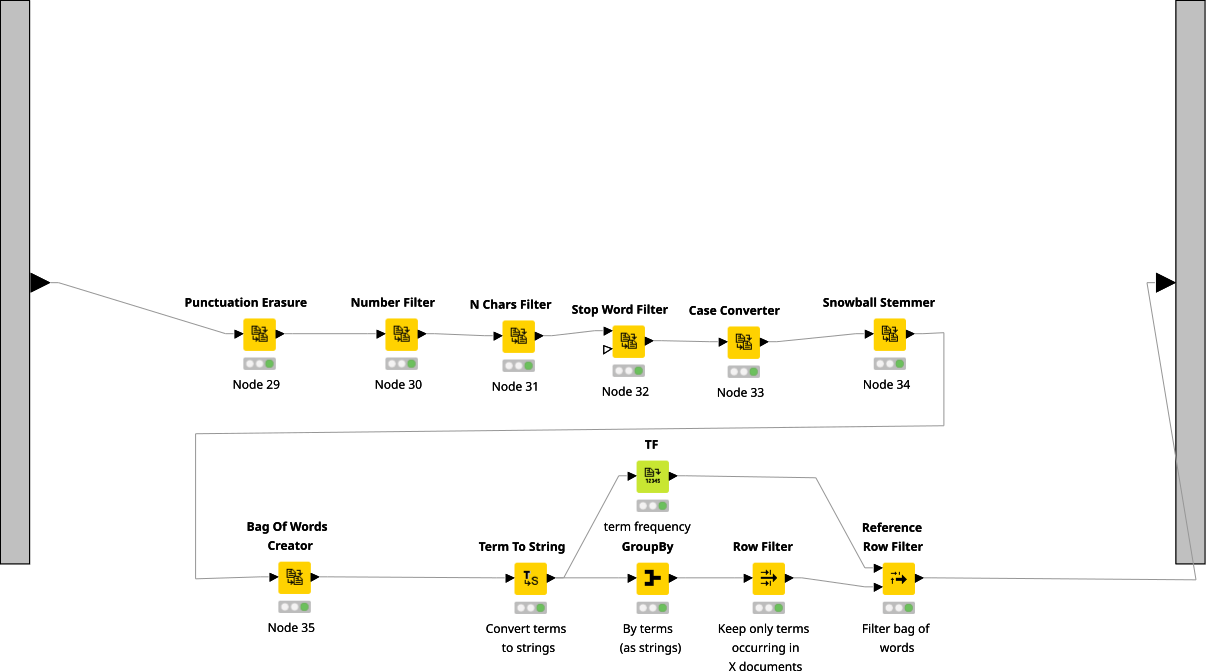
\includegraphics[width = \textwidth]{preprocesamiento.png}
	\caption{Preprocesamiento aplicado a los documentos para modelos de clasificación.}
	\label{fig:preprocesamiento}
\end{figure}


Como vemos, simplemente limpiamos los documentos de caracteres especiales, palabras muy cortas, y pasamos todas las palabras a minusculas. Tras esto nos quedamos con los términos más frecuentes, que será con los que trabajemos.

\section{Uso de métodos de clasificación}

Una vez realizado el preprocesamiento simplemente separamos los documentos en entrenamiento y test, y aplicamos los métodos de clasificación.

En mi caso he escogido utilizar los clasificadores Random Forest y Logistic Regression:

\begin{figure}[H]
	\centering
	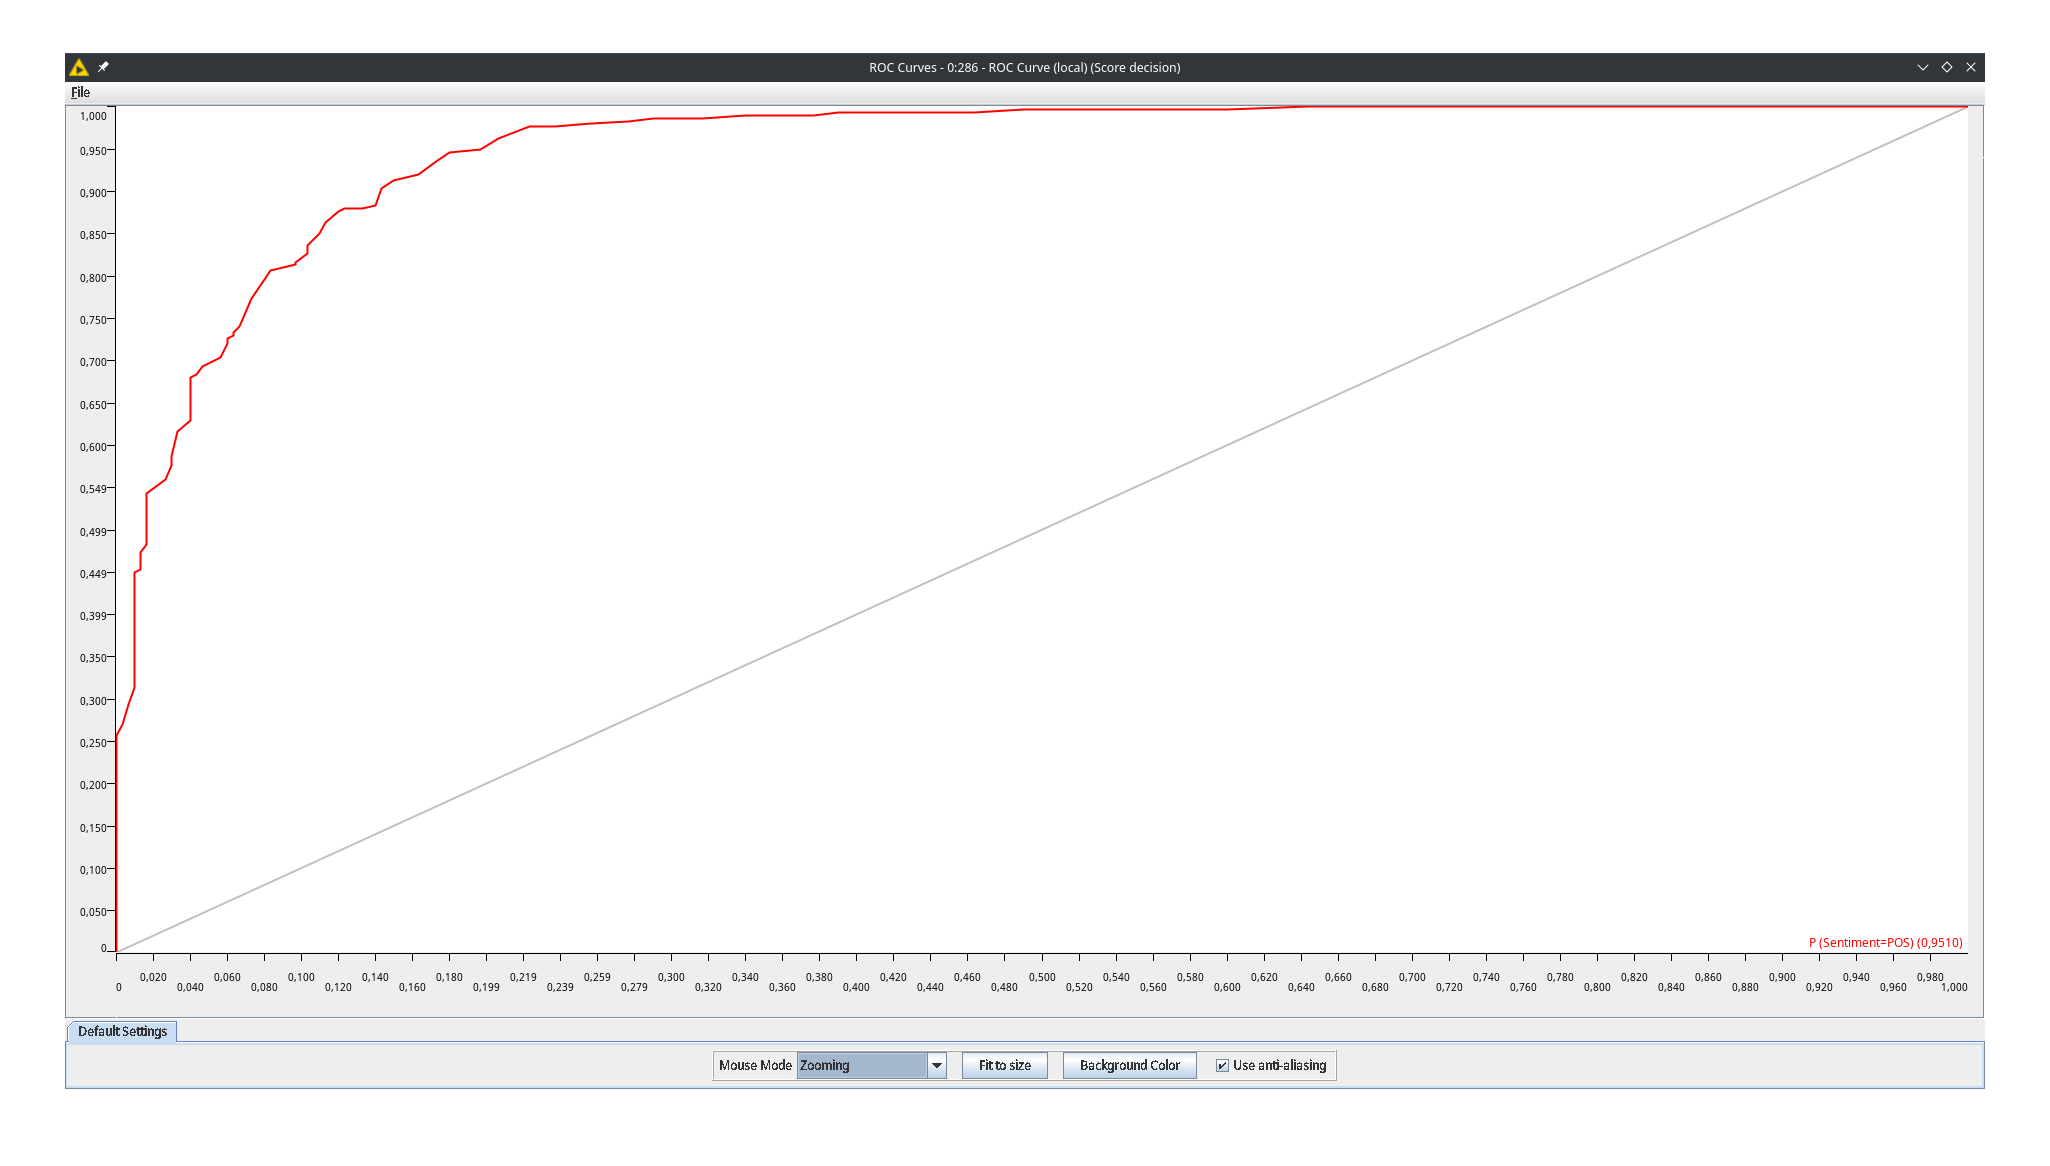
\includegraphics[width = \textwidth]{roc_RF.png}
	\caption{Curva ROC obtenida del modelo Random Forest.}
	\label{fig:roc_RF}
\end{figure}

\begin{figure}[H]
	\centering
	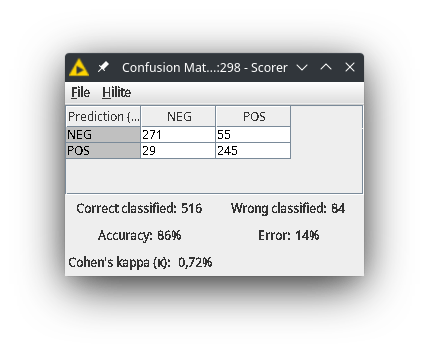
\includegraphics[width = \textwidth]{matriz_RF.png}
	\caption{Matriz de confusión obtenida del modelo Random Forest.}
	\label{fig:matriz_RF}
\end{figure}

\begin{figure}[H]
	\centering
	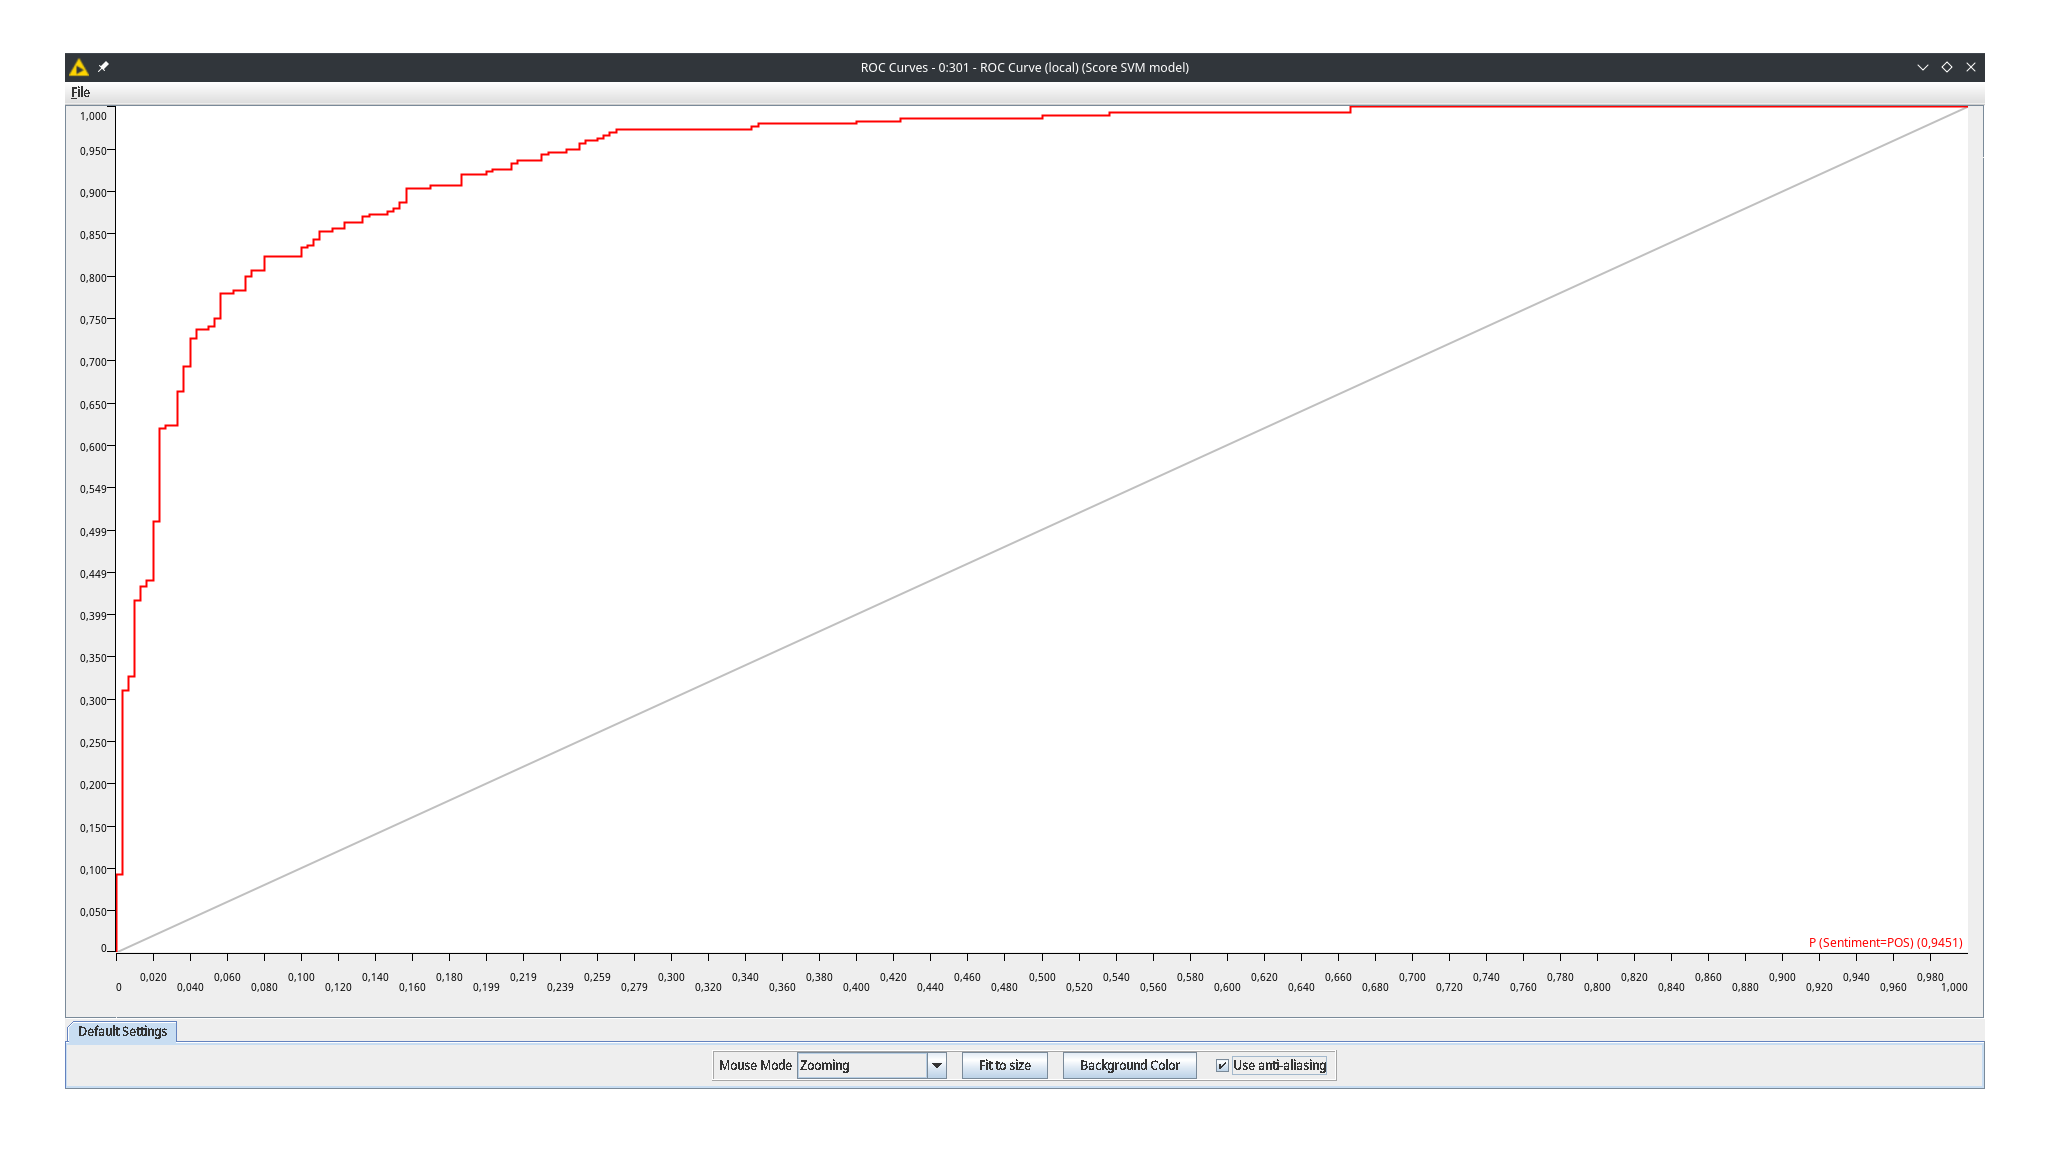
\includegraphics[width = \textwidth]{roc_LR.png}
	\caption{Curva ROC obtenida del modelo Logistic Regression.}
	\label{fig:roc_LR}
\end{figure}

\begin{figure}[H]
	\centering
	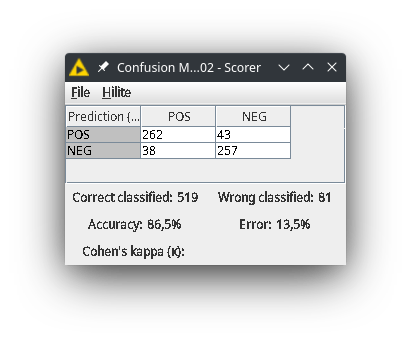
\includegraphics[width = \textwidth]{matriz_LR.png}
	\caption{Matriz de confusión obtenida del modelo Logistic Regression.}
	\label{fig:matriz_RL}
\end{figure}

Como vemos, con ambos modelos conseguimos resultados similares, alrededor del 85-90\% de acierto, una tasa de acierto bastante buena. Vamos comparar estos resultados con utilizar diccionarios.


\section{Uso de diccionarios para análisis de sentimientos}

El uso de diccionarios para predecir opiniones se basa en, a cada palabra, asociar una opinión positiva o negativa, y contar si en un documentos existen más palabras positivas o negativas.

Para comenzar, la primera tarea es leer dichos diccionarios.

\subsection{Lectura de diccionarios}

\subsection{Uso para decidir el sentimiento de documentos}


\section{Comparación entre uso de modelos de clasificación y de diccionarios}


\section{Workflow final}


El flujo final realizado a lo largo de la práctica es el siguiente:

\begin{figure}[H]
	\centering
	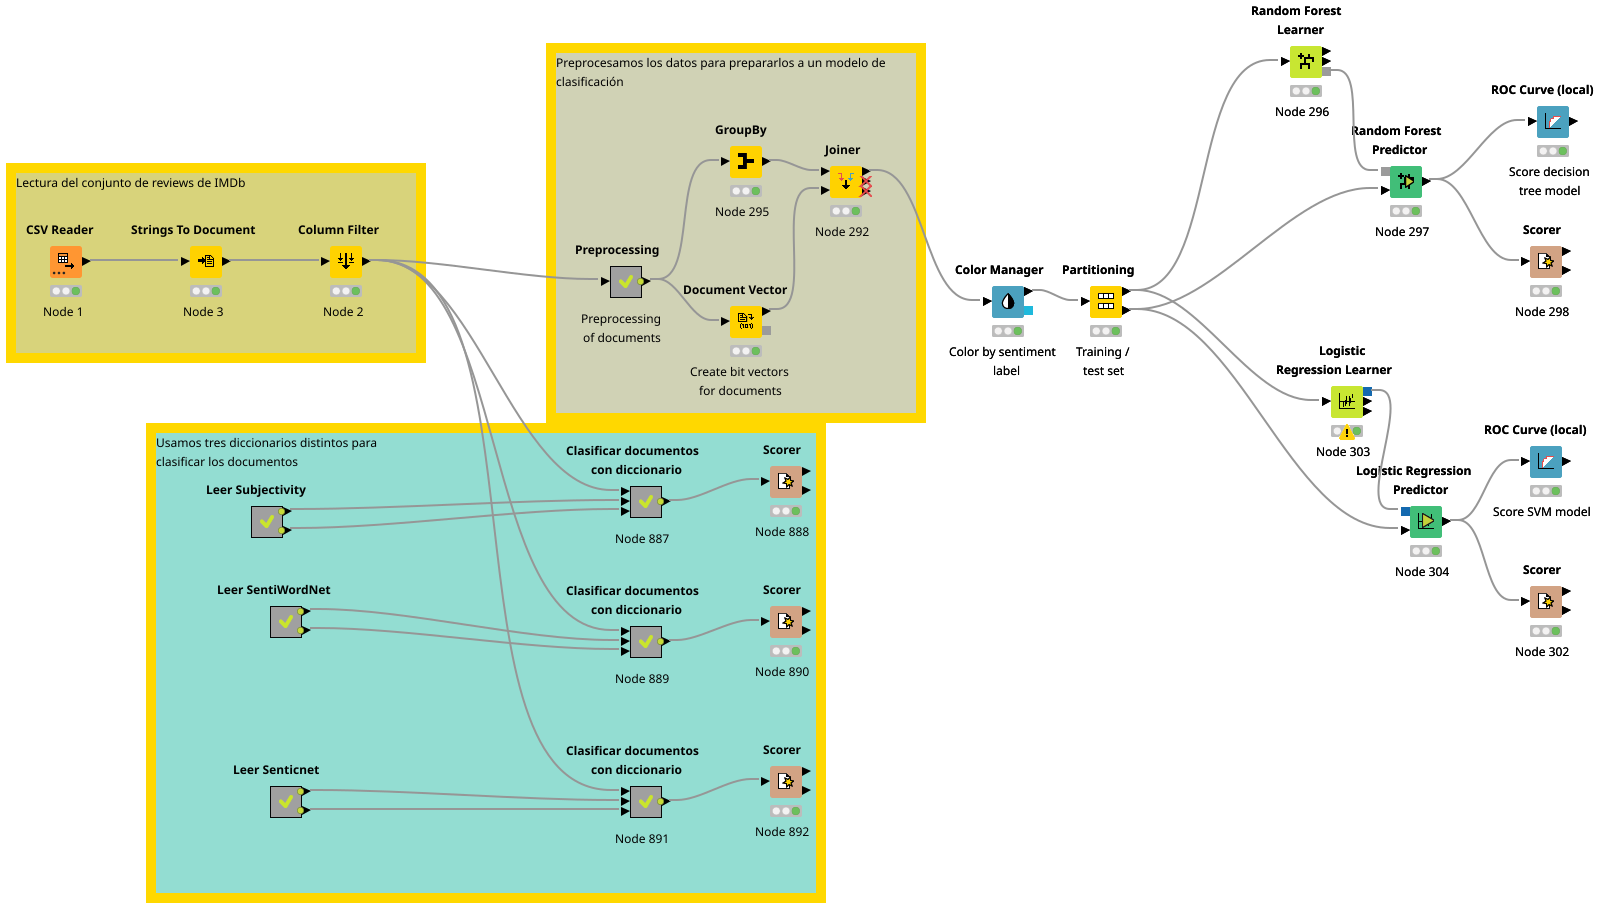
\includegraphics[width = \textwidth]{workflow_knime.png}
	\caption{Workflow final de KNIME.}
	\label{fig:workflow_knime}
\end{figure}
